\documentclass[a4paper,11pt]{jsarticle}


\usepackage{amsmath,amsthm,amsfonts,float,cases,bm,amssymb,amssymb,ascmac}
\usepackage[dvipdfmx]{graphicx}
\usepackage[all]{xy}
\usepackage{makeidx}
\makeindex

\setlength{\textwidth}{\fullwidth}
\setlength{\textheight}{40\baselineskip}
\addtolength{\textheight}{\topskip}
\setlength{\voffset}{-0.55in}

\newtheorem{thm}{定理}[section]
\newtheorem{cor}[thm]{系}
\newtheorem{dfn}[thm]{定義}
\newtheorem{lem}[thm]{補題}
\newtheorem{rem}[thm]{注意}
\newtheorem{eg}[thm]{例}


\begin{document}
\date{}
\title{ホモトピー論の基本について}

\maketitle
\begin{abstract}
  ホモトピー論の基本について網羅的に書いたものではなく,勉強中に特に注意して考えたことをまとめたもの.
\end{abstract}
\tableofcontents
\section{ホモトピー群}
\subsection{相対ホモトピー群の4種類の定義}
4種類の相対ホモトピー群の定義を述べる.絶対バージョンに対しても同じことが言えるが,自然に同一視できるいろいろな定義をinterchangeablyに使えるようになりたい場面,例えば自分にとって慣れている定義とは異なる定義を採用している論文を読むときなどのために,各定義の関係を把握しておくと便利だと思う.また,幾何学的直感の働きやすい定義と,理論的に便利なabstractな定義の間の関係を把握しておくとabstractな対象に対する直感も育まれるとおもう.そのための備忘録,チートシートとしてこの小節を用意する.
\paragraph{一つ目の定義(cubeを使った定義)}
$I^n$の部分空間$J^n$を\index{$J^n$}$J^n:=\partial I^{n-1}\times I\cup I^{n-1}\times\{0\}$と定める.$n=1,\ 2,\ 3$の場合を書けばその形はわかる.$n=1$の場合$\{0\}$,$n=2$の場合上が空いたコの字型($\sqcup$),$n=3$の場合上の開いた箱型である.

\index{きてんつきくうかんつい@基点付き空間対}\textgt{基点付き空間対}$(X,A,*)$とは空間対$(X,A)$と$A$の点$*\in A$の組のことである.このとき,$n>0$に対し
\footnote{$n=0$の場合でも定義は可能だが,$I^0={0},\ \partial I^0=\varnothing,\ J^0=\varnothing$ゆえ,絶対バージョンと同じになる.}
$(X,A,*)$の\index{ほもとぴーぐん@($n$次)ホモトピー群}\textgt{$n$次ホモトピー群}\index{pinXAstar@$\pi_n(X,A,*)$}$\pi_n(X,A,*)$を3対のホモトピー集合\[
  \pi_n(X,A,*):=[(I^n,\partial I^n,J^n),(X,A,*)]
\]と定める.基点が文脈から明らかな時は\index{pinXA@$\pi_n(X,A)$}$\pi_n(X,A)$と書く.
この定義から,$\pi_n(X,A,*)$の元の代表元$f,g\colon I^n\to X$が等しいための条件はホモトピー$h\colon I^n\times I\to X$で,次を満たすものが存在することである.\[
  任意のt\in Iとx\in \partial I^n,\ y\in J^nに対し,h(x,t)\in Aかつh(y,t)=*.
\]
ホモトピー群の元の代表元は空間の3対の連続写像であるという条件から,その像は$n=2$の場合例えば以下の絵(この絵の場合,$D^2$と同相なものの絵を描いているつもりである.
もちろんこんなにきれいに行かない場合がほとんどである!)のようになる.
$J^n$を1点につぶすことにより空間の3対の同相$(I^n,\partial I^n,J^n)\cong(D^n,S^n,*)$を得るので.ホモトピー群はこの同相を通じて$[(D^n,S^n,*),(X,A,*)]$と同一視できる.

\begin{figure}[h]
  \centering
  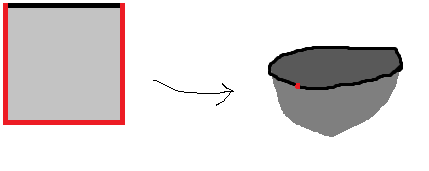
\includegraphics[]{I^2.png}
\end{figure}
\paragraph{群構造}
$n\ge 2$に対し\footnote{$n=1$だと,道の終点が$A$に含まれることしか保証されていないので,「道をつなぐ」ことが自然に定義できない.例えば$A$が2点集合だった場合を考えればわかる.},$\pi_n(X,A)$に群構造を入れる.
$f,g\colon (I^n,\partial I^n,J^n)\to (X,A,*)$に対し,その積$f\cdot g\colon (I^n,\partial I^n,J^n)\to (X,A,*)$を,\[
  (f\cdot g)(t_1,\dots,t_n):=\left\{
  \begin{alignedat}{5}
    &f(2t_1&&,t_2,\dots,t_n)\ \ &&(0&&\le t_1\le 1/2&&)\\
    &g(2t_1-1&&,t_2,\dots,t_n)\ \ &&(1/2&&\le t_1\le 1&&)
  \end{alignedat}\right.
\]と定めると,写像空間$\mathrm{Map}((I^n,\partial I^n,J^n),(X,A,*))$に$H$-spaceの構造が入る(略).よってホモトピー群に群の構造が入る.また$n\ge 3$なら$\pi_n(X,A)$はAbel群である.可換なことの証明は絶対バージョンと同様である.$n=2$だと可換とは限らないのはなぜか.$\pi_1(X)$が可換とは限らないという事実よりも非自明に思えるので,もう少しちゃんと考えたい(@TODO).$X:=(D^2\vee D^2,S^1\vee S^1)$への2種類の標準的なinclusion\ $i_1,i_2\colon(D^2,S^1)\hookrightarrow X$の積$i_1\cdot i_2$と$i_2\cdot i_1$の間に基点を止めた相対ホモトピーがなさそうなのでそれで理解できそうだが$\dots$(これこそ障害理論の適用例として使える?).
\begin{figure}[h]
  \centering
  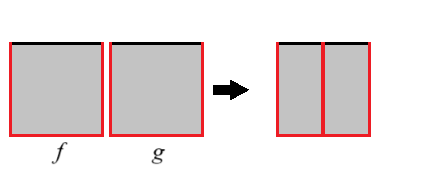
\includegraphics{defOfHomotopyGroup_composition.png}
\end{figure}

\paragraph{二つ目の定義(discを使った定義)}@TODO $I^n$を$D^n$に置き換えた場合にpinch mapおよびfoldingmapを導入し,上の定義とは少し異なる幾何学的直感を与える,しかし同一視できる群構造の入れ方を具体的に書き下しておく.
\paragraph{三つ目の定義(homotopy fiberの$n-1$次loopspaceの$0$次ホモトピー群)}@TODO loop spaceに標準的な積が定まり,それが$H$-spaceになることを述べた後$\pi_n(X,A):=\pi_0(\Omega^{n-1}(\mathrm{Path}(X,{*},A)))$と定める.
\paragraph{四つ目の定義(homotopy fiberの$n-1$次ホモトピー群)}@TODO inclusion $A\hookrightarrow X$のホモトピーファイバーの$n-1$次ホモトピー群を$n$じ相対ホモトピー群として定める.loop spaceの性質をいくつか使えば三つ目のとほぼ同じに見える.
\paragraph{すべての定義を自然に同一視できること}4つの定義によって作られた相対ホモトピー群の間に自然な同型を構成する.面倒だが,いろんな定義をinterchangeablyに使えることと,その間の同型を具体的に知っておくこと,また幾何学的に絵で理解できる定義とabstractに作られた定義の間の対応を具体的に見ておくことで,abstractな対象に対する直感ができることは重要だと思うのでやる.
\subsection{Hurewiczの定理}
\subsection{Freudenthalの懸垂定理}
\subsection{Whiteheadの定理}
\section{局所係数の(コ)ホモロジー}
\subsection{局所系の2種類の定義}
\subsection{局所係数の(コ)ホモロジーの計算例}
\section{障害理論}
\subsection{CW複体上の写像を延ばせるかどうかのcriterion}
\subsection{E-M空間}

\printindex





\end{document}